\documentclass[11pt,a4paper]{article}

% --- Packages (mirrors Project 1) ---
\usepackage[utf8]{inputenc}
\usepackage[T1]{fontenc}
\usepackage{amsmath,amssymb}
\usepackage{graphicx}
\usepackage[margin=2.5cm]{geometry}
\usepackage{booktabs}
\usepackage{hyperref}
\usepackage{caption}
\usepackage{subcaption}
\usepackage{siunitx}
\usepackage{natbib}
\usepackage{float}

\graphicspath{{fig/}}
\bibliographystyle{unsrtnat}

\title{Monte Carlo Simulation of the Two-Dimensional XY Model}
\author{Zhaoyang Chu \\ s4390199
        \and
        Zoutong Shen \\ s4879759 \\[6pt]
        Computational Physics 2026 --- Project 2 --- Group 12}
\date{\today}

\begin{document}
\maketitle

% ============================================================
% ABSTRACT  [Report structure 10%]
% ============================================================
\begin{abstract}
% TODO Pass 2: write abstract (~150 words). Cover:
%   - 2D XY model on N x N square lattice, Metropolis Monte Carlo,
%     periodic boundary conditions, J1 = k_B = 1
%   - what we measured: <|m|>, <e>, chi_M, C, tau, vortex counts
%   - validation: two-starts equilibration; chi_M peak vs Hasenbusch
%     T_BKT = 0.8935
%   - extension: NNN diagonal coupling J2/J1 = 0.5 shifts the transition
%     up and suppresses vortices
%   - one sentence on the main numerical takeaway
\end{abstract}

% ============================================================
% 1  INTRODUCTION / BACKGROUND  [Theoretical background 10%]
% ============================================================
\section{Introduction}
\label{sec:introduction}

% TODO Pass 2: motivate the 2D XY model.
%   - Continuous O(2) spin model, simplest setting where Mermin-Wagner
%     forbids true LRO at T > 0 in 2D yet a topological transition still
%     occurs (BKT)
%   - Vortex unbinding picture; quasi-LRO below T_BKT
%   - Goal: simulate, measure all standard observables, compare to
%     literature, then extend with a next-nearest-neighbour coupling
%   - Last paragraph: roadmap of the remaining sections, mirroring
%     Project 1's "the rest of this paper is organised as follows"

\subsection{The XY Model and the BKT Transition}
\label{sec:xy_model}

% TODO Pass 2:
%   - Spin variable s_i = (cos theta_i, sin theta_i)
%   - Hamiltonian: H = -J_1 sum_<i,j> cos(theta_i - theta_j)
%     (introduce J_2 only later in Section sec:extension)
%   - Mermin-Wagner: continuous symmetry plus short-range interaction
%     in 2D forbids spontaneous breaking; spin-wave expansion gives
%     <s(0).s(r)> ~ r^{-eta(T)} (algebraic / quasi-LRO)
%   - BKT picture: bound vortex/anti-vortex pairs at low T, unbinding
%     transition at T_BKT; for J = 1 the high-precision value is
%     T_BKT = 0.8935 (cite hasenbusch2005)
%   - eta(T_BKT) = 1/4 quoted for context, not measured here
%   - Cite kosterlitz1973, mermin1966

\subsection{Vortices and Topological Charge}
\label{sec:vortices_theory}

% TODO Pass 2:
%   - Definition of plaquette winding number: sum of four nearest-
%     neighbour angle differences around a 2x2 plaquette, each wrapped
%     into (-pi, pi], divided by 2 pi
%   - Result is integer: +1 (vortex), -1 (anti-vortex), 0 elsewhere
%   - On a periodic lattice the total topological charge sums to zero
%     (n_+ = n_-): a sanity check on the detector
%   - Below T_BKT vortices are bound in pairs (low density); above T_BKT
%     they unbind (proliferate) -- we will see this in Section sec:vortices
%   - Cite tobochnik1979 for the plaquette definition

\subsection{Observables}
\label{sec:observables}

% TODO Pass 2: define everything we measure, with formulae:
%   - per-spin magnetisation m = |M| / N^2 with M = sum_i s_i
%   - per-spin energy e = E / N^2
%   - magnetic susceptibility chi_M = (1 / N^2) * (<M^2> - <M>^2) / k_B T
%     = beta * N^2 * var(m)
%   - specific heat per spin C = (1 / N^2) * (<E^2> - <E>^2) / (k_B T)^2
%     = N^2 * var(e) / T^2
%   - autocorrelation function chi(t) and integrated correlation time tau
%     (defined fully in Section sec:error_analysis)

% ============================================================
% 2  METHODS
% ============================================================
\section{Methods}
\label{sec:methods}

\subsection{Metropolis Algorithm}
\label{sec:metropolis}

% TODO Pass 2:
%   - One MC sweep = N^2 single-spin trial moves (so each spin gets one
%     attempted update per sweep on average, independent of N)
%   - Trial proposal: pick a site (r, c) uniformly; propose
%     theta' = theta + delta * u with u ~ U(-1, 1), delta = pi
%   - Metropolis accept/reject: min(1, exp(-beta * Delta E))
%   - Delta E depends only on the chosen spin and its 4 nearest neighbours
%     (8 if J_2 != 0); local energy is O(1) per move
%   - Total energy E and components M_x, M_y are tracked incrementally
%     from the sweep deltas, which avoids O(N^2) recomputation
%   - Cite metropolis1953

\subsection{Equilibration and Sampling Protocol}
\label{sec:protocol}

% TODO Pass 2:
%   - For each (T, N) we start from an ordered configuration (theta = 0
%     at every site), run n_equil sweeps and discard them, then run
%     n_prod sweeps recording |M|/N^2 and E/N^2 every sweep
%   - Production lengths used in this report:
%       N = 50 main scan: n_equil = 2000, n_prod = 30000 sweeps
%       N = 20 (J_2 extension only): n_equil = 2000, n_prod = 20000 sweeps
%   - Time unit: one MC sweep
%   - Temperature scan: 11 values at T = 0.5, 0.7, ..., 2.5 (step 0.2),
%     comfortably above the rubric's "at least 10" requirement
%   - State that the validation in Section sec:validation justifies the
%     choice of n_equil

\subsection{Error Analysis}
\label{sec:error_analysis}

% TODO Pass 2:
%   - Autocorrelation function:
%       chi(t) = <m(t') m(t' + t)> - <m(t')><m(t' + t)>
%     using matched-subset means so chi(0) = var(m) (eq. 2 of lecture 8)
%   - Integrated correlation time: tau = sum_{t=0}^{t*} chi(t) / chi(0),
%     with t* the first lag where chi turns negative (lecture 8 cutoff
%     to avoid the noisy tail)
%   - Standard error of a correlated mean:
%       sigma = sqrt( 2 tau / N_samples * var(m) )
%   - Susceptibility and specific heat from fluctuations:
%       chi_M = beta * N^2 * var(m_per_spin)
%       C     = N^2 * var(e_per_spin) / T^2
%   - Blocking method for chi_M and C errors: split production into
%     non-overlapping blocks of length 16 * tau, evaluate the estimator
%     on each block, take the standard error of the block values
%   - Cite newman1999 and cmph_lecture8

\subsection{Vortex Detection}
\label{sec:vortex_detection}

% TODO Pass 2:
%   - For each 2x2 plaquette walk a -> b -> c -> d -> a and sum the four
%     angle differences wrapped into (-pi, pi]
%   - Divide by 2 pi and round to integer => topological charge
%     +1 (vortex), -1 (anti-vortex), 0 (smooth plaquette)
%   - Reference vortices.py:plaquette_charges for the implementation
%   - Cite tobochnik1979

% ============================================================
% 3  RESULTS
% ============================================================
\section{Results}
\label{sec:results}

\subsection{Validation}
\label{sec:validation}

% TODO Pass 2 -- state the goal: prove the simulation is correct before
% interpreting any physics. Three independent checks below.

\subsubsection{Equilibration: Two Starts}
\label{sec:two_starts}

% TODO Pass 2:
%   - Show ordered- and random-start time series at the same temperature
%     converge to the same plateau in |m| and e
%   - Comment on equilibration time and confirm n_equil = 2000 sweeps is
%     comfortably enough
%   - Discuss the harder case at T = 2.5 (deeply disordered): both starts
%     lose memory of the initial condition quickly

\begin{figure}[H]
    \centering
    \begin{subfigure}{0.49\textwidth}
        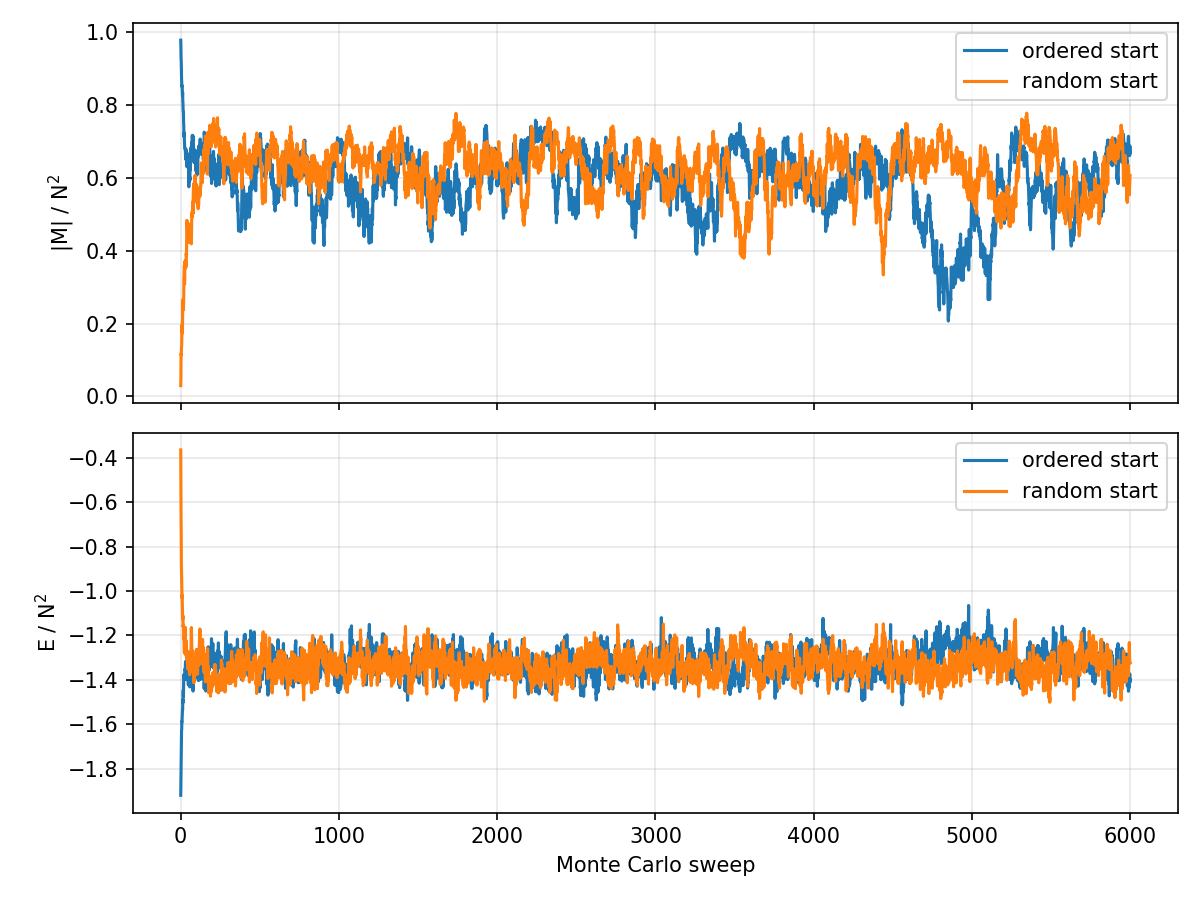
\includegraphics[width=\linewidth]{two_starts_N20_T1.00.png}
        \caption{TODO Pass 2: ordered vs random start at $T = 1.0$ (near $T_{\mathrm{BKT}}$), $N = 20$.}
        \label{fig:two_starts_T1}
    \end{subfigure}
    \hfill
    \begin{subfigure}{0.49\textwidth}
        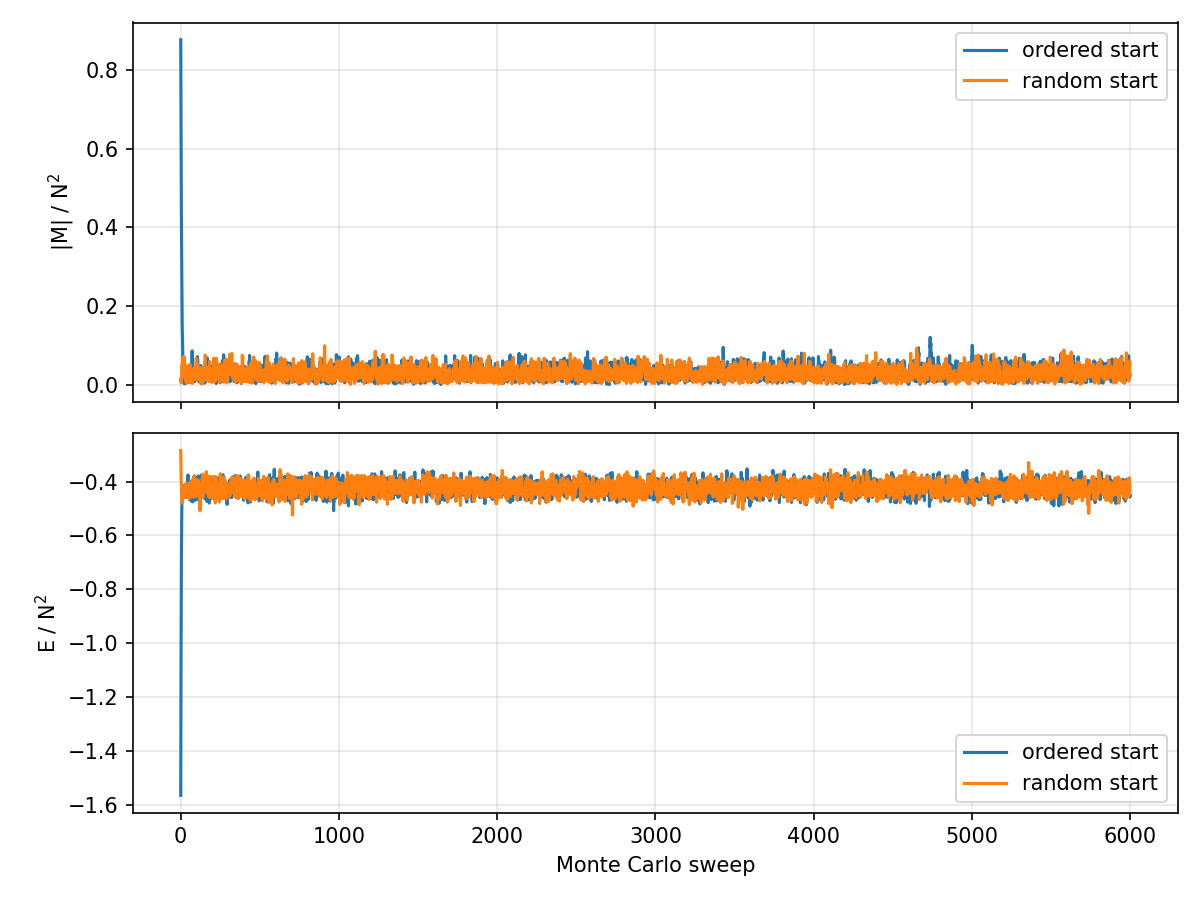
\includegraphics[width=\linewidth]{two_starts_N50_T2.50.png}
        \caption{TODO Pass 2: ordered vs random start at $T = 2.5$ (deep disordered phase), $N = 50$.}
        \label{fig:two_starts_T2.5}
    \end{subfigure}
    \caption{TODO Pass 2: equilibration validation. Two independent starts at the same temperature converge to the same plateau in $|m|$ and $e$, demonstrating that the simulation is sampling the equilibrium distribution.}
    \label{fig:two_starts}
\end{figure}

\subsubsection{Stationarity: Single-run Trace}
\label{sec:trace}

% TODO Pass 2:
%   - Show |m| and e are stationary after equilibration
%   - Mention visible autocorrelation in the trace and connect it to the
%     correlation time tau computed in Section sec:correlation

\begin{figure}[H]
    \centering
    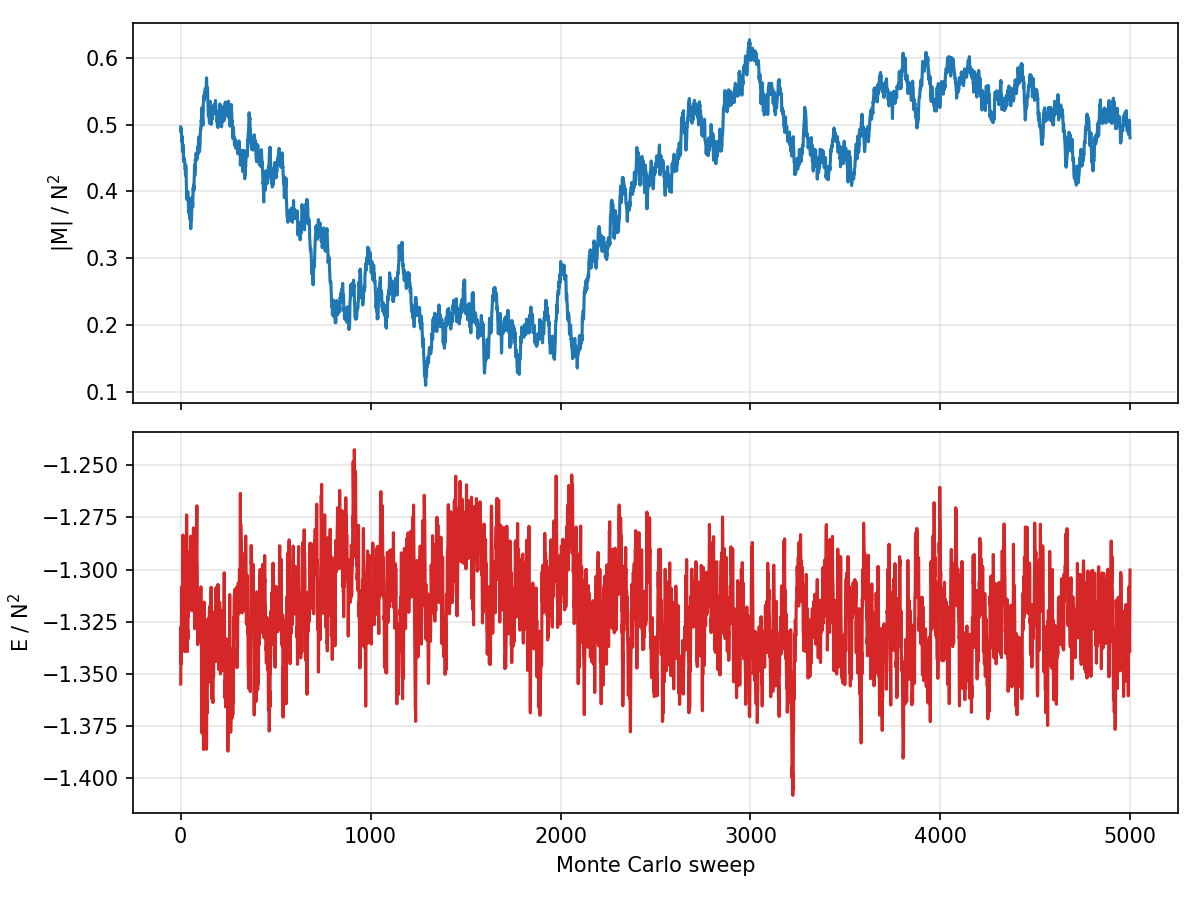
\includegraphics[width=0.8\textwidth]{time_series_N50_T1.00.png}
    \caption{TODO Pass 2: production trace of $|m|$ and $e$ at $T = 1.0$, $N = 50$.}
    \label{fig:trace}
\end{figure}

\subsubsection{Critical Temperature vs Literature}
\label{sec:tc_validation}

% TODO Pass 2:
%   - Read off the chi_M peak temperature T_chi from the N = 50 scan
%     (Section sec:magnetisation, Figure fig:scan_main top-right)
%   - Compare to Hasenbusch's high-precision T_BKT = 0.8935 (cite
%     hasenbusch2005)
%   - Discuss the upward finite-size shift: chi_M peak temperature
%     decreases monotonically toward T_BKT as N grows; small N over-
%     estimates the transition slightly (textbook BKT finite-size
%     behaviour)
%   - Numbers go in the summary table in Section sec:summary_table

\subsubsection{Finite-size Sanity}
\label{sec:fs_sanity}

% TODO Pass 2:
%   - Briefly show that scan_N50 has sharper, more localised peaks in
%     chi_M and C than scan_N20 (already in figures), confirming the
%     expected sharpening with N

\subsection{Magnetisation and Susceptibility}
\label{sec:magnetisation}

% TODO Pass 2:
%   - Plot <|m|>(T) and chi_M(T) (top row of fig:scan_main)
%   - <|m|> does not drop sharply to zero -- consistent with no LRO at
%     T > 0 (Mermin-Wagner) and with the finite-size rounding of the
%     BKT transition
%   - chi_M shows a clear peak at T_chi ~ T_BKT
%   - Error bars: correlated SE on <|m|>, blocking error on chi_M

\subsection{Energy and Heat Capacity}
\label{sec:energy}

% TODO Pass 2:
%   - Plot <e>(T) and C(T) (bottom row of fig:scan_main)
%   - <e>(T) is smooth and monotonic (no latent heat: BKT is essential)
%   - C(T) has a finite peak slightly above T_BKT -- well-known feature,
%     not a divergence
%   - Error bars: correlated SE on <e>, blocking error on C

\begin{figure}[H]
    \centering
    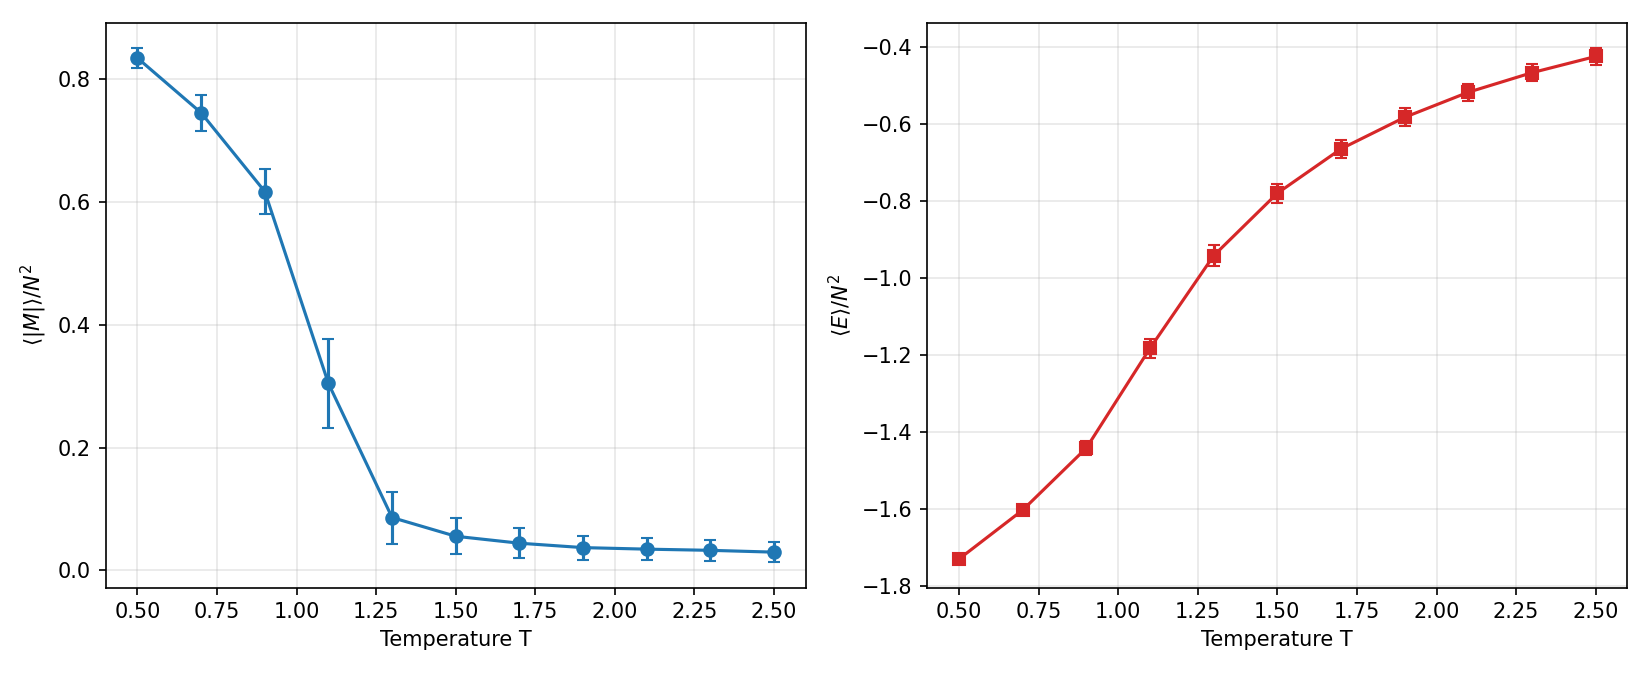
\includegraphics[width=\textwidth]{scan_N50.png}
    \caption{TODO Pass 2: temperature dependence of $\langle |m| \rangle$, $\langle e \rangle$, $\chi_M$, and $C$ for the $N = 50$ scan. Error bars: correlated standard error on the means, blocking method on $\chi_M$ and $C$.}
    \label{fig:scan_main}
\end{figure}

\subsection{Correlation Function and Correlation Time}
\label{sec:correlation}

% TODO Pass 2:
%   - Two figures address the rubric phrase "correlation function as a
%     function of temperature":
%       (a) chi(t)/chi(0) vs lag t at T = 0.5, 0.9, 2.1 -- the
%           autocorrelation FUNCTION, showing slow decay at T ~ T_BKT
%           and fast decay in the ordered/disordered phases
%       (b) tau(T) at all 11 scan temperatures -- the integrated
%           correlation TIME, peaking near T_BKT (critical slowing down)
%   - Discuss critical slowing down and how the peak in tau motivates
%     the 16 tau block length used for chi_M and C error bars

% TODO Pass 2: this figure requires a new --mode autocorrelation in
% plot_results.py that calls analysis.autocorrelation on the |M|/N^2
% series for a few representative temperatures. Once added, generate
% with:
%   python plot_results.py --mode autocorrelation \
%       --input data/scan_N50.npz \
%       --output figures/autocorrelation_curves_N50.png
% Then uncomment the figure block below.
%
% \begin{figure}[H]
%     \centering
%     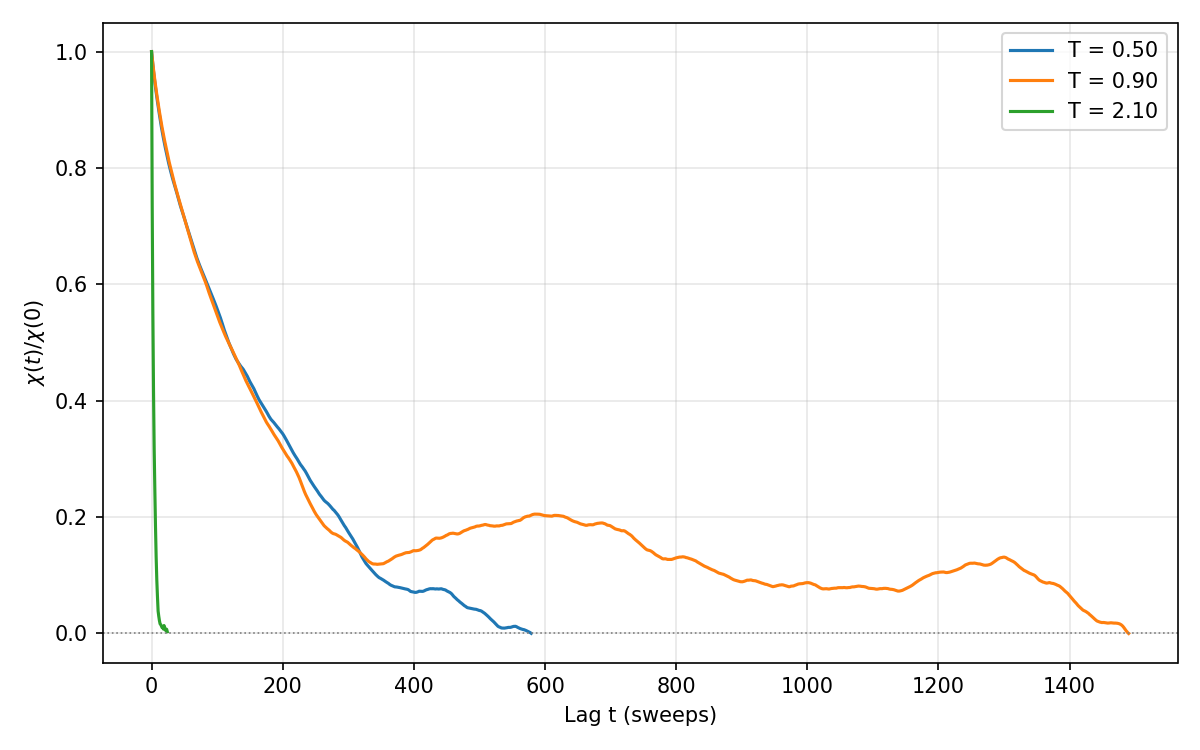
\includegraphics[width=0.8\textwidth]{autocorrelation_curves_N50.png}
%     \caption{TODO Pass 2: normalised autocorrelation function $\chi(t)/\chi(0)$ of $|m|(t)$ at three representative temperatures, $N = 50$.}
%     \label{fig:autocorr}
% \end{figure}

% TODO Pass 2: regenerate at N = 50 from data/scan_N50.npz; placeholder
% for now is the existing N = 20 figure.
\begin{figure}[H]
    \centering
    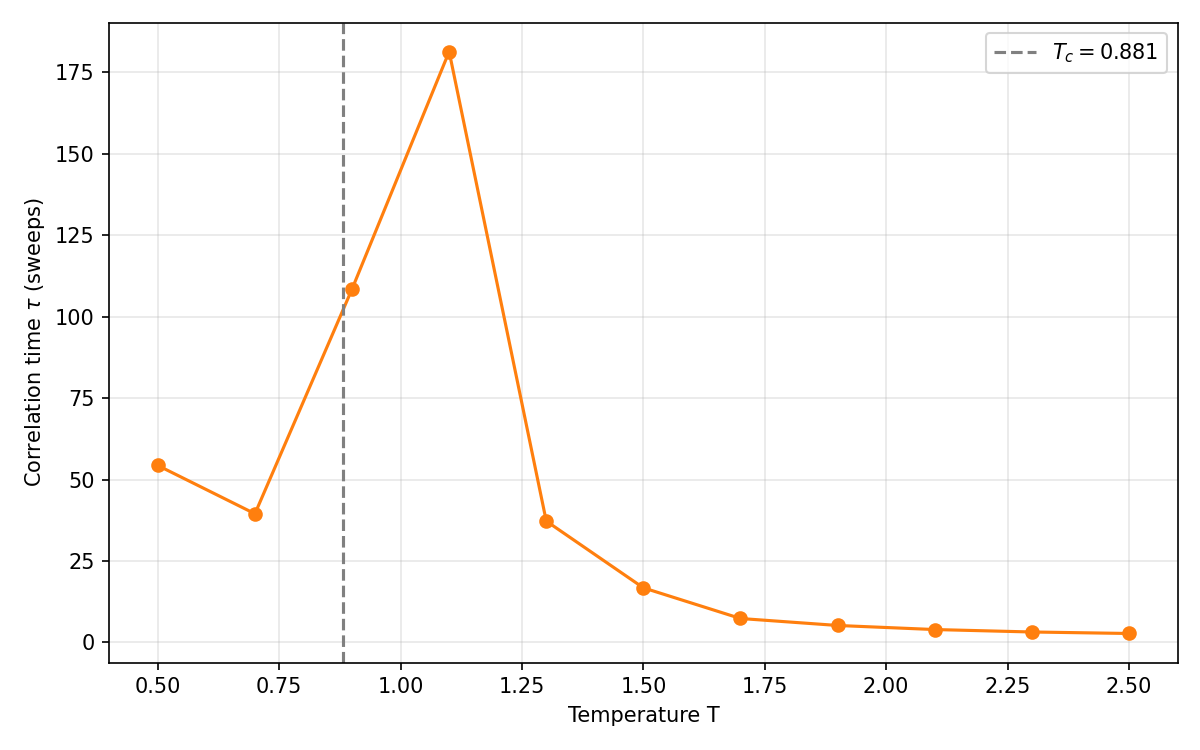
\includegraphics[width=0.7\textwidth]{tau_N20.png}
    \caption{TODO Pass 2: integrated correlation time $\tau(T)$ at $N = 50$ across the 11 scan temperatures (placeholder shows $N = 20$ until regeneration).}
    \label{fig:tau}
\end{figure}

\subsection{Vortices at Low Temperature}
\label{sec:vortices}

% TODO Pass 2:
%   - Visual: configuration_vortices_N30_T1.00.png shows isolated bound
%     vortex/anti-vortex pairs at T just above T_BKT
%   - Quantitative: vortex count vs T flat-low at T < T_BKT, rising
%     rapidly through and above T_BKT (unbinding picture)
%   - Note that n_+ = n_- exactly on the periodic lattice (detector sanity
%     check)
%   - Optional contrast: vectors_N50_T2.00.png in the deep disordered
%     phase -- vortices everywhere, no orientational order

\begin{figure}[H]
    \centering
    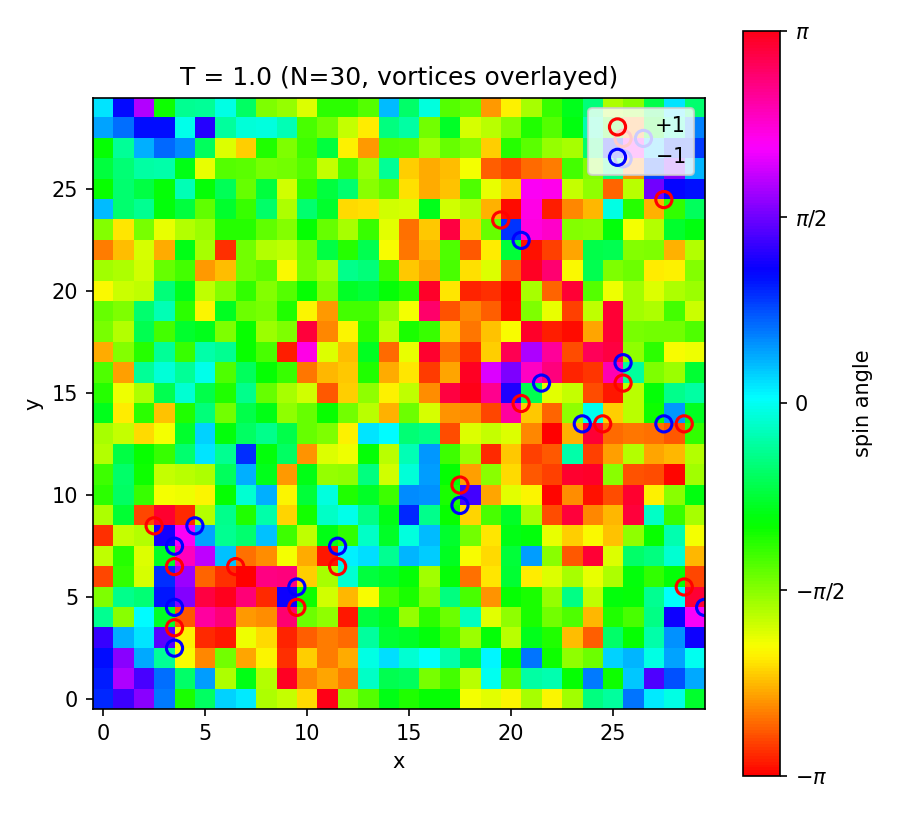
\includegraphics[width=0.6\textwidth]{configuration_vortices_N30_T1.00.png}
    \caption{TODO Pass 2: spin configuration at $T = 1.0$, $N = 30$, with $+1$ vortices (red) and $-1$ anti-vortices (blue) circled. Bound pairs are visible.}
    \label{fig:vortex_config}
\end{figure}

% TODO Pass 2: regenerate at N = 50; placeholder shows N = 20.
\begin{figure}[H]
    \centering
    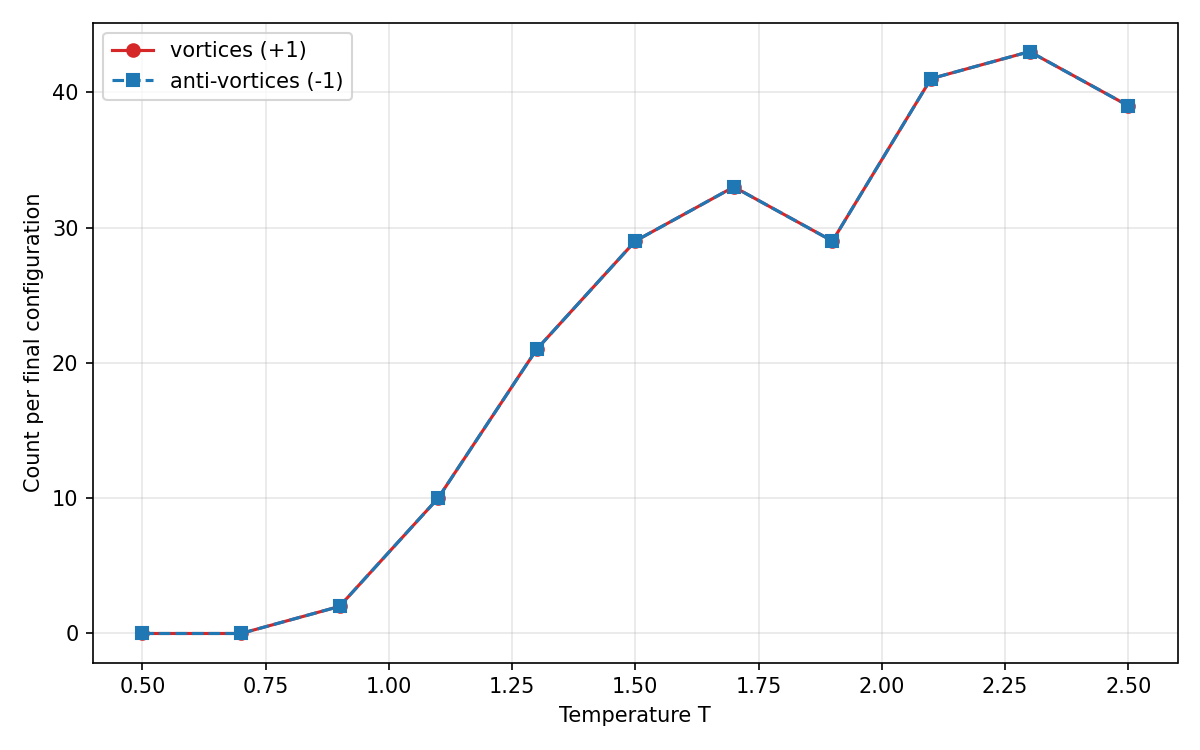
\includegraphics[width=0.7\textwidth]{vortex_count_N20.png}
    \caption{TODO Pass 2: number of $+1$ vortices and $-1$ anti-vortices in the final configuration as a function of $T$, $N = 50$ (placeholder shows $N = 20$). On a periodic lattice the two counts coincide.}
    \label{fig:vortex_count}
\end{figure}

\subsection{Configuration Grid}
\label{sec:config_grid}

% TODO Pass 2:
%   - One paragraph walking through scan_configurations_N50.png:
%       low T: nearly aligned, few vortices
%       T ~ T_BKT: large smooth domains separated by isolated vortex
%                  pairs
%       high T: fully disordered, dense vortex lattice
%   - This is the visual summary of all the quantitative results

\begin{figure}[H]
    \centering
    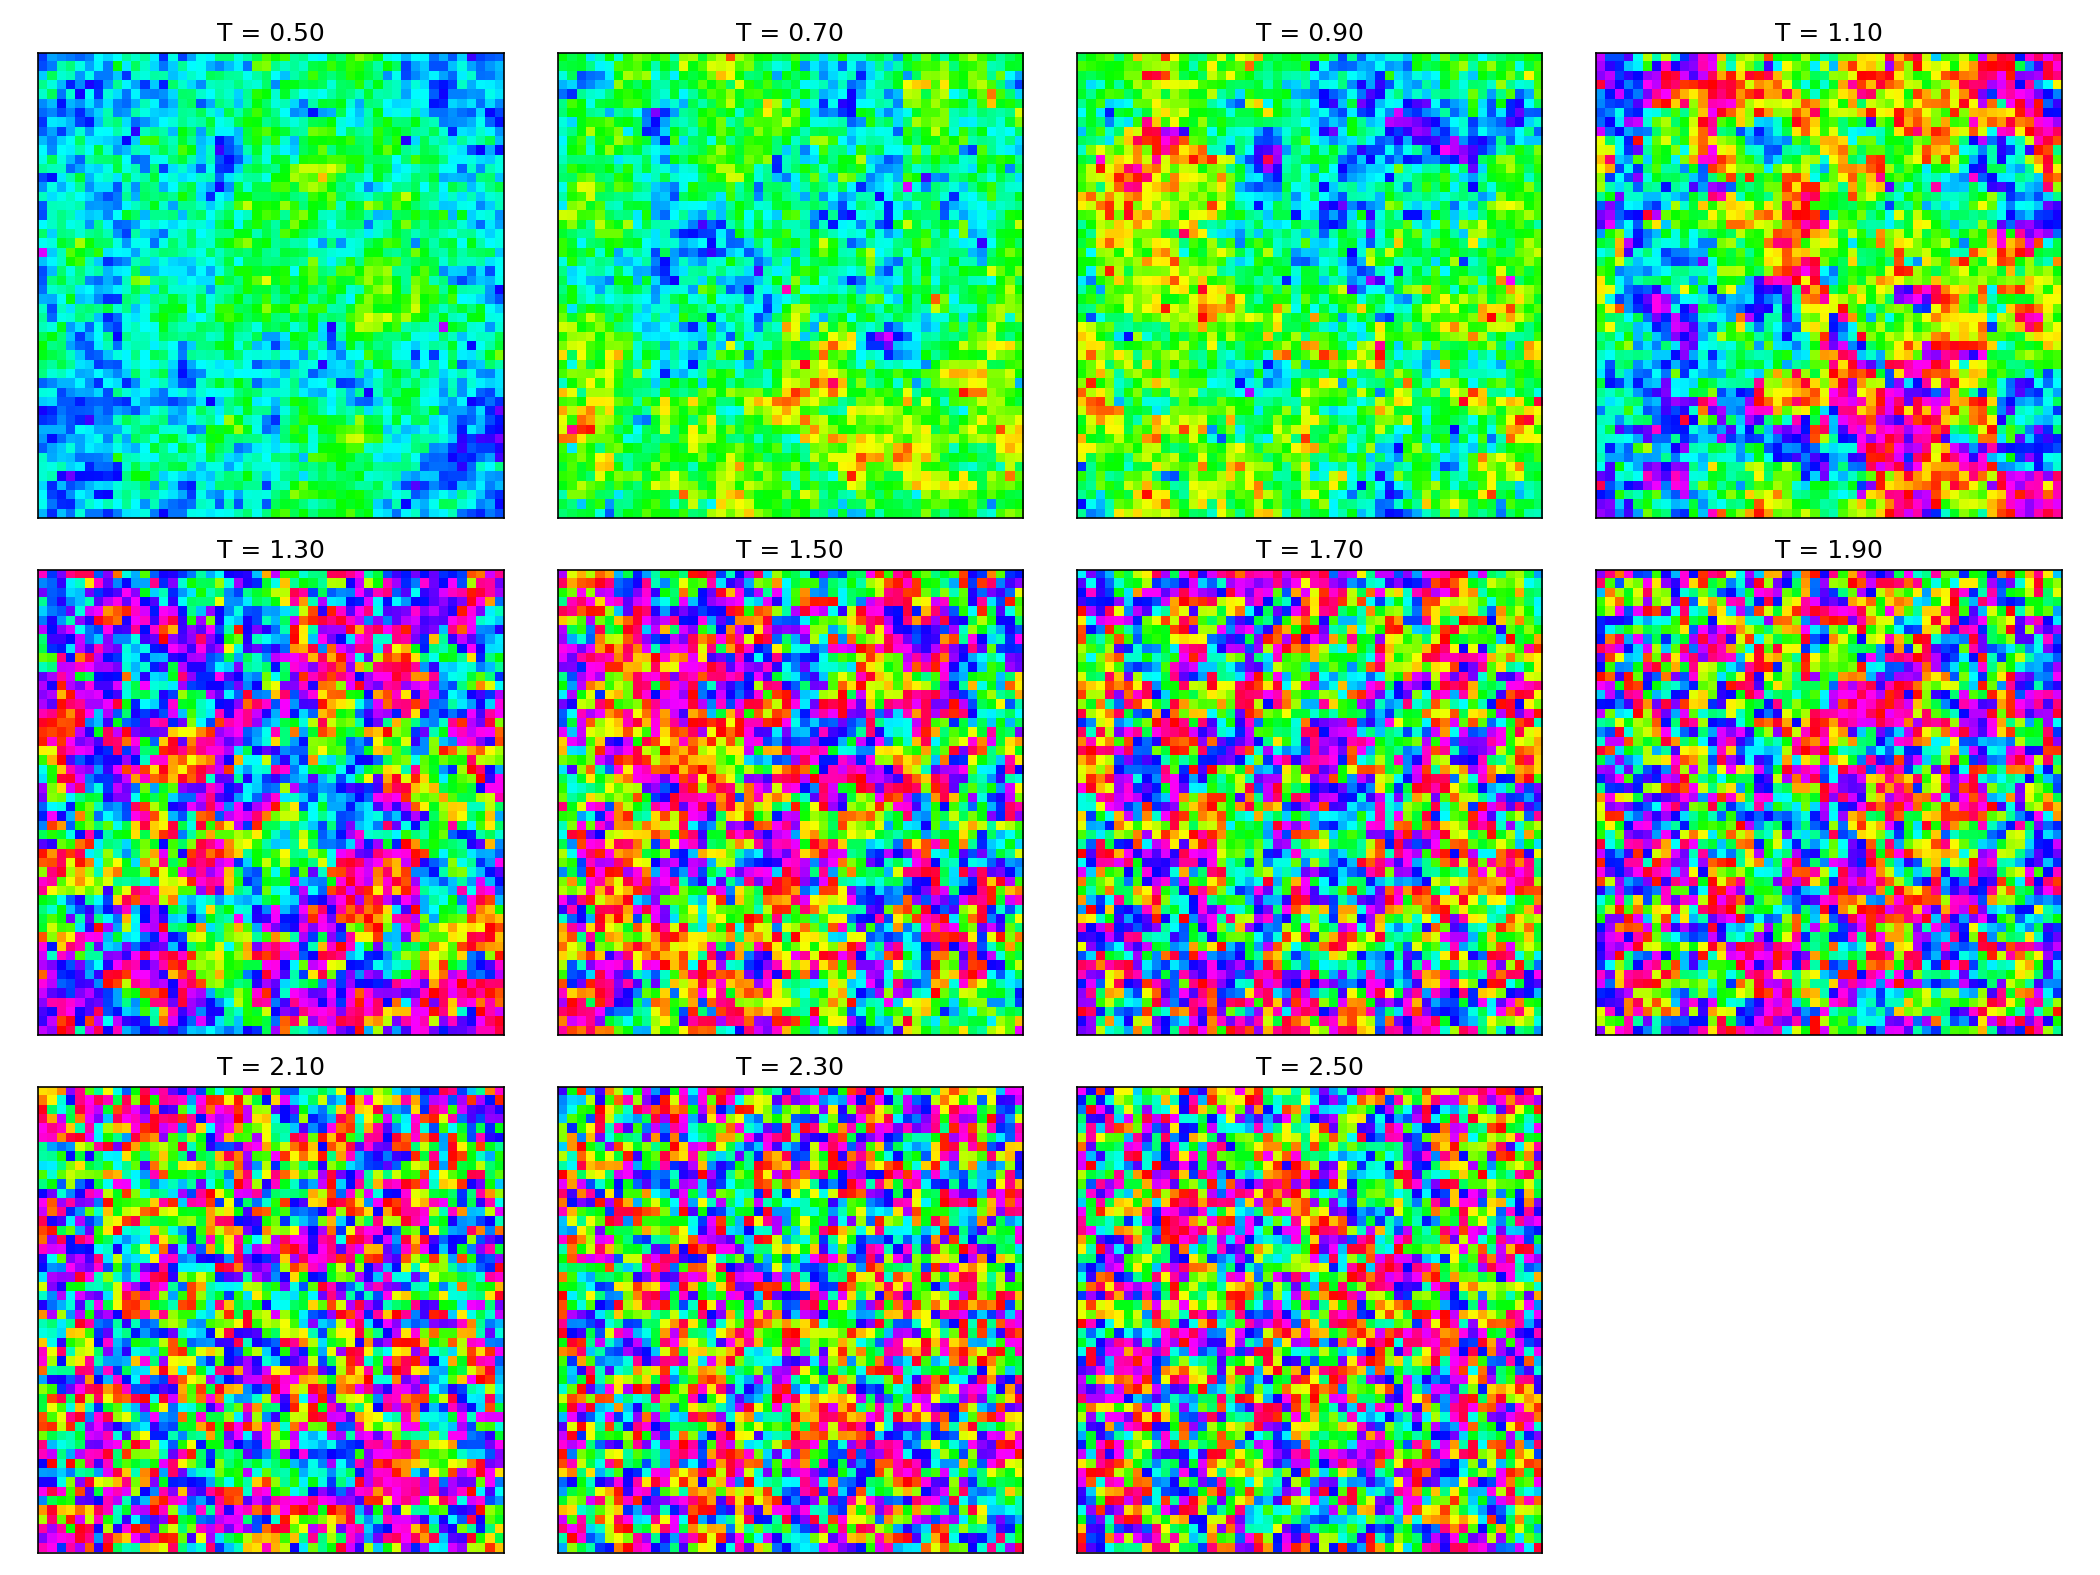
\includegraphics[width=\textwidth]{scan_configurations_N50.png}
    \caption{TODO Pass 2: final spin configurations across the temperature scan, $N = 50$, with hue encoding the spin angle.}
    \label{fig:config_grid}
\end{figure}

\subsection{Numerical Summary}
\label{sec:summary_table}

% TODO Pass 2: fill in the table with numbers read off the N = 50 scan
% (analysis.scan_statistics output). Numbers below are placeholders.

\begin{table}[H]
    \centering
    \caption{TODO Pass 2: peak quantities from the $N = 50$ temperature scan, with the literature comparison.}
    \label{tab:summary}
    \begin{tabular}{lcc}
        \toprule
        Quantity                              & Value                & Source \\
        \midrule
        $T$ at $\chi_M$ peak                  & TBD $\pm$ TBD        & this work, $N = 50$ \\
        $\chi_M$ at peak                      & TBD $\pm$ TBD        & this work, $N = 50$ \\
        $T$ at $C$ peak                       & TBD $\pm$ TBD        & this work, $N = 50$ \\
        $C$ at peak                           & TBD $\pm$ TBD        & this work, $N = 50$ \\
        Literature $T_{\mathrm{BKT}}$         & $0.8935$             & \citet{hasenbusch2005} \\
        Relative deviation of $T_{\chi}$      & TBD\,\%              & this work vs literature \\
        \bottomrule
    \end{tabular}
\end{table}

% ============================================================
% 4  EXTENSION  [Extension 10%]
% ============================================================
\section{Extension: Next-Nearest-Neighbour Diagonal Coupling}
\label{sec:extension}

\subsection{Motivation and Hamiltonian}
\label{sec:ext_motivation}

% TODO Pass 2:
%   - Add diagonal NNN bonds with coupling J_2 along (+/-1, +/-1) on top of
%     the J_1 nearest-neighbour bonds
%   - Full Hamiltonian:
%       H = -J_1 sum_<i,j> cos(theta_i - theta_j)
%           -J_2 sum_<<i,j>> cos(theta_i - theta_j)
%   - Run with J_2 / J_1 = 0.5 (--j2-ratio 0.5)
%   - Expected effects: more ferromagnetic coupling => T_BKT shifts up,
%     vortex cores cost more energy, configurations are smoother at fixed T,
%     <e> is more negative at every T

\subsection{Method Changes}
\label{sec:ext_method}

% TODO Pass 2:
%   - Single new local term per site (xy_simulation.py:local_energy and
%     xy_simulation.py:total_energy already gated by j2_ratio != 0)
%   - At j2_ratio = 0 the trajectory is bit-identical to the J_1-only
%     simulation for the same seed -- a regression guarantee noted in
%     the README

\subsection{Results}
\label{sec:ext_results}

% TODO Pass 2:
%   - Headline figure (compare_scans_N20.png): 2x3 panel overlaying both
%     scans -- <|m|>(T), <e>(T), tau(T), chi_M(T), C(T), vortex count
%   - Quote the chi_M peak shift: T = 1.1 (J_2 = 0) -> T = 1.9 (J_2 = 0.5)
%     at N = 20 (verify against the actual figure when writing prose)
%   - Energy is more negative everywhere
%   - Vortices are suppressed at fixed T
%   - One paragraph relating the J_2 effect to the spin-stiffness picture
%     of BKT: more bonds per site => higher stiffness => higher T_BKT

\begin{figure}[H]
    \centering
    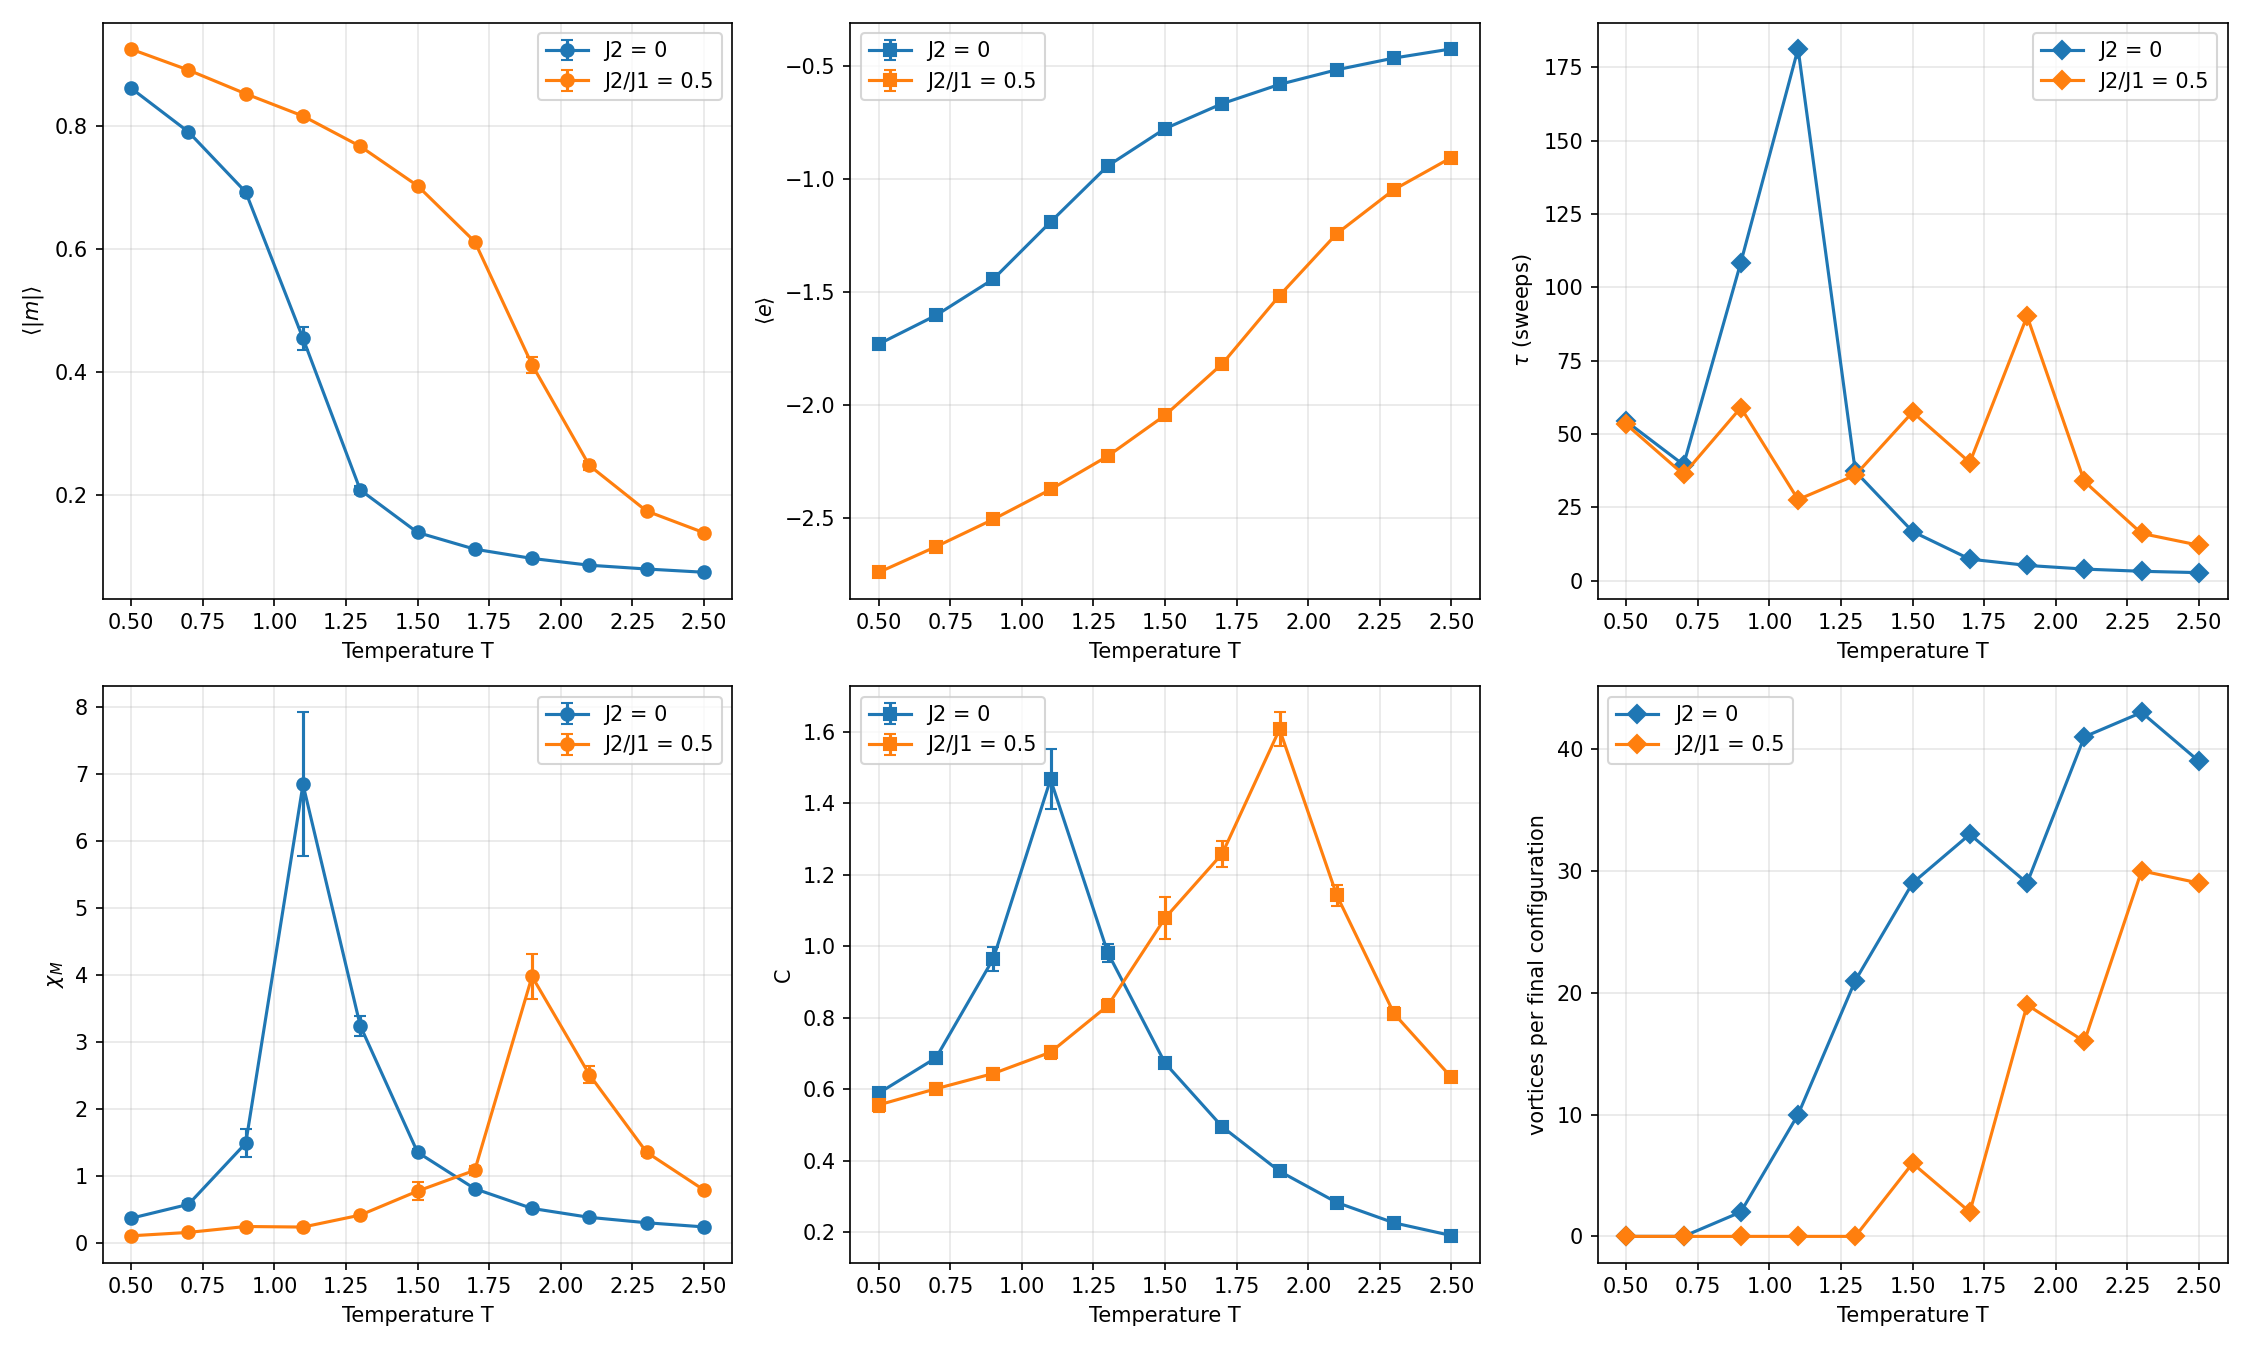
\includegraphics[width=\textwidth]{compare_scans_N20.png}
    \caption{TODO Pass 2: $J_1$-only vs $J_1 + J_2$ comparison at $N = 20$ for $\langle |m| \rangle$, $\langle e \rangle$, $\tau$, $\chi_M$, $C$, and the vortex count.}
    \label{fig:compare_scans}
\end{figure}

\begin{figure}[H]
    \centering
    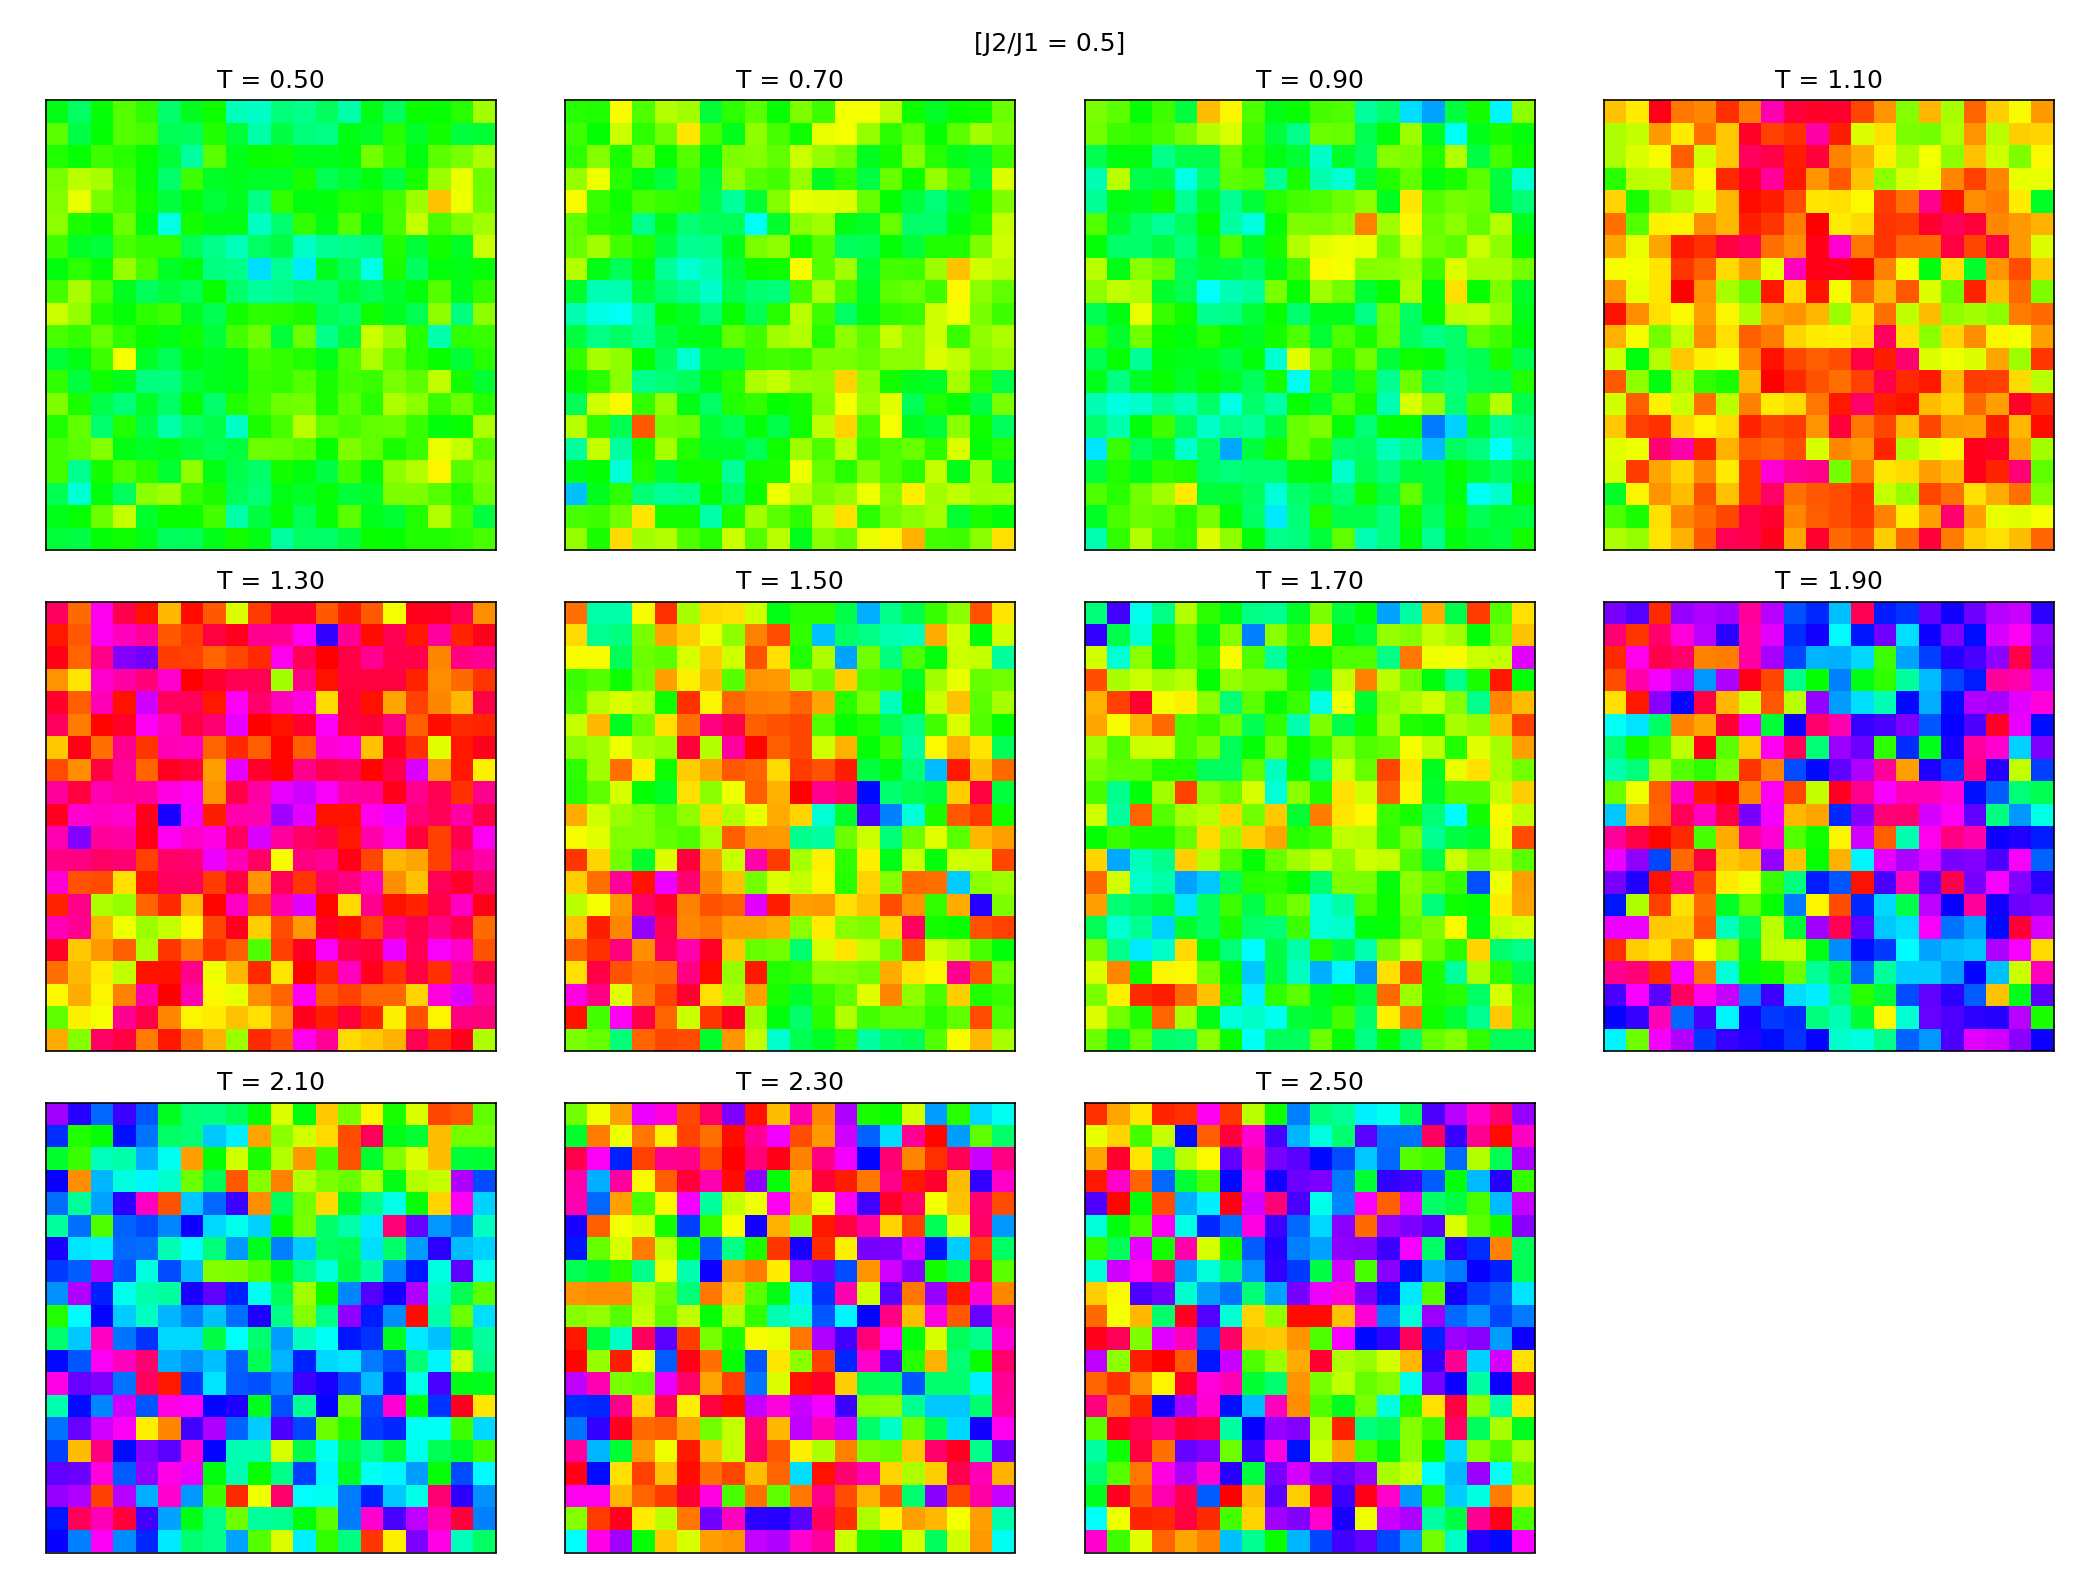
\includegraphics[width=\textwidth]{scan_configurations_N20_j2_0.50.png}
    \caption{TODO Pass 2: final spin configurations across the temperature scan with $J_2 / J_1 = 0.5$, $N = 20$. Smoother than the $J_2 = 0$ case at matched $T$.}
    \label{fig:config_grid_j2}
\end{figure}

% ============================================================
% 5  SUMMARY
% ============================================================
\section{Summary}
\label{sec:summary}

% TODO Pass 2:
%   - One paragraph: what was built (Metropolis MC of the 2D XY model,
%     observable suite, vortex detector, J_2 extension)
%   - One paragraph: main numerical results (T_chi vs Hasenbusch, peak
%     locations of chi_M and C, vortex behaviour)
%   - One paragraph: extension takeaway (J_2 shifts T_BKT up, suppresses
%     vortices at fixed T)
%   - Limitations: small N (no proper finite-size scaling extrapolation,
%     no eta(T) measurement), Metropolis only (no Wolff cluster updates
%     to beat critical slowing down), no off-diagonal correlation function
%     measurement

% ============================================================
% REFERENCES
% ============================================================
\bibliography{references}

\end{document}
